\chapter{Introduction}
\thispagestyle{chapterBeginStyle}

\begin{center}
    \textit{ "Let's have a beer!" }
\end{center}

From the scenario of buying a beer we will go through the whole process of designing what is called Credential System. After few initial questions and considerations, we state the key requirements of the system and later a proposition of solution is presented.

Let us think about the beer for a moment, about the process of buying it in particular. Bob goes to the bar, greets the bartender and asks for his favourite flavor of beer. According to the Polish law, it is illegal to sell alcohol to the underage, so not to get into any trouble the worker wants to verify his "entitlement". Most often he does it by checking it with any of Bob's identification documents. If he approves that the person on the photo is really Bob and the date of birth yields the proper age,  he sells the beverage Bob came there to buy.

This is so trivial that we hardly ever think about this, almost no one notices that the bartender now also knows the 
data that was on ID. If we consider the identification document issued about five years ago, the bartender had additional access to name and surname, address of residence, names of parents, height and eye color, ID serial number and PESEL number. That's actually a lot of information especially that those information have nothing to do with ability to buy a drink. We might argue that in such a short it is impossible for the bartender to actually remember all the additional information, but still, it creates a risk. One last thing, notice that the bartender had access to exact date of birth while the only thing he should be curious about is just the question if Bob is above the required age or not. The knowledge he possess might be used to send Bob a birthday gift or next time ask about parents by their name, but more possibly the bartender would use this information to gain unfair advantage or use it in a malicious way.

If one has any concerns about privacy some questions should arise in his head. Is it possible to just show the attributes that are required? How can one mask his actual date of birth and just proof the fact that he is allowed to drink? Is it possible to do it in the way, that next time the bartender will not be able to link Bob's previous purchases with this one?

This simple and somehow amusing scenario should shine some light on what we want to achieve in the design of Credential System. Privacy is the main concern, but we cannot forget about usability or efficiency. General overview of Credential System and its requirements are presented in next sections.

\clearpage

\section{Motivation}

The key reason for a credential system is to enhance (or actually introduce) the control over disclosure of authenticated data.
If we think about data as an attributes that have some properties (e.g. age is a number from some range) most of the time for verification only some of those properties have to be checked. It is commonly done by just showing the data and the verifying entity checks if the conditions are met, but it does not have to be that way. One can prove some facts about possessed data without revealing them and this is one of the key arguments for the design of Credential System (i.e. one can prove he is at least 18 years old, but does disclose the exact age).

Identity Mixer \cite{idemix} by IBM is one of the proposed solutions to the considered problem. It allows to authenticate without disclosing any personal data, thus, no personal data is collected and allows to minimize the personal data they have to reveal.

Our design of the Credential System (CreS) aims to achieve similar functionality as the one developed by IBM but by employing different and more efficient cryptographic structures. 

\section{Credential System Overview}

The Credential System usually consists of three parties:
\begin{itemize}
    \item \textbf{User} is the holder of credentials and corresponding attributes (like name, age, address etc.).
    \item \textbf{Issuer} is an entity that verifies the attributes and issues the credential to the user.
    \item \textbf{Verifier} verifies the validity of credential but does not learn the value of attributes. 
\end{itemize}
The overview of interactions between Credential System parties is presented on figure \ref{fig: credential system overview} % todo figure

\begin{figure}[h]
\centering
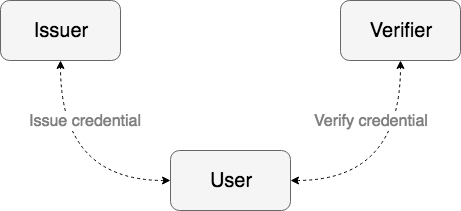
\includegraphics[scale=0.6]{images/CredentialSystemDiagram.png}
\caption{Overview of Credential System}
\label{fig: credential system overview}
\end{figure}

\noindent The \textbf{Credential} is an object with which the user may prove his qualities or entitlements, which may have following properties:
\begin{itemize}
    \item Does not reveal signed attributes to the verifying entity. 
    \item The verifier cannot link multiple presentations of the same credential.
    \item Can be issued under masked attributes (e.g. private keys, sensitive data etc.)
\end{itemize}

Description provided here should serve as general intuition of the system, more in-depth definitions and requirements will be provided in later parts of this paper. One should remember that although the formal definitions will build the cryptographic base of the system, the idea of what the system should do, and the motivation behind the need for such system, should be understood intuitively. 


\section{Use Cases}

Apart from the example from the introduction we can consider following scenarios:
\begin{itemize}
    \item \textbf{Room access system}
    
    Opening doors by presenting proper credential with possible option to make tracking users infeasible. Access rights and restrictions are naturally present in form of an attribute.
    \item \textbf{Bus ticket system}
    
    Verification does not require presentation of other IDs, and does not leak any information about communication patterns.
    \item \textbf{Online Movie Subscription}
    
    The only thing that gets verified is if one have valid subscription.
    \item \textbf{Driving license}
    
    Understood as driving permission ("this person is allowed to drive this kind of vehicle") without disclosing sensitive information.
\end{itemize}

The scenarios are endless and only on the need depend how they could be solved. The motivation of this paper is to equip the people in tools necessary to create such working and secure Credential System. The operational requirements of the system are presented in next section.


\section{System Requirements}
Below we present general requirements of the Credential System.

\begin{itemize}
    \item \textbf{Credential unforgeability}
    
    It should be infeasable for any number of colluding parties to obtain a valid credential without consent of the issuer.
    \item \textbf{Attributes privacy} 
    
    If should be infeasable for any number of colluding parties to obtain value of hidden attributes, without the owner reveling them.
    \item \textbf{Computational effectiveness}
    
    Performed computations should be possibly efficient and require small storage size without compromising security.
    \item \textbf{Transparency}
    
    System should be possibly simple and transparent from the user's perspective.
    \item \textbf{Modularity}
    
    System should be compact, extendable and ready for integration with similar existing systems.
\end{itemize}
Additionally, the system might provide:
\begin{itemize}
    \item \textbf{Multiple-show unlinkability}
    
    It should be infeasable for any number of colluding parties to link multiple presentations of the same credential. This considers only the attributes that are meant to be hidden. If we consider the case of linking users to the pseudonyms in domains it is natural to expect such possibility.
    
    \item \textbf{Non-transferability}
    
    It should be infeasable for any number of colluding parties to transfer a valid credential between different users without sharing all credential data (all or nothing).
\end{itemize}


% \section{Structure of this Document}
% In section ...
% In section

% What might be skipped and why
% What parts are the core of this document
